\documentclass[eng,openany]{mgr}
\usepackage{listings}
\usepackage[english]{babel}
\usepackage{graphicx}
\usepackage{hyperref}
\usepackage{tabularx,colortbl} 
\usepackage{rotating}
\usepackage[utf8]{inputenc} 
\usepackage{amssymb}
\setlength\parindent{24pt}
\usepackage[parfill]{parskip}
\usepackage[table,kernelfbox,hyperref]{xcolor}
\usepackage{fancyhdr}
\usepackage{gauss}
%\usepackage[colorinlistoftodos]{todonotes}

\hypersetup{colorlinks=true}
\hypersetup{xurlbordercolor=red!70!black}
\hypersetup{xlinkbordercolor=blue!70!black}
\hypersetup{linkcolor=blue!60!black}
\hypersetup{urlcolor=red!50!black}
\hypersetup{citecolor=green!30!black}
\rfoot{Page \thepage}
\renewcommand\lstlistlistingname{List of Listings}
\newcommand{\linia}{\rule{\linewidth}{0.4mm}}

\definecolor{listlightgray}{gray}{0.93}

\newcommand{\lstsetmylst} {
\lstset{frame = tb,
breaklines=true,
framerule = 0.25pt,
float,
fontadjust,
backgroundcolor={\color{listlightgray}},
basicstyle = {\ttfamily\footnotesize},
identifierstyle = {\ttfamily},
stringstyle = {\ttfamily},
showstringspaces = false,
showtabs = false,
numbers = left,
numbersep = 6pt,
tabsize = 4,
language=C,
floatplacement=!h
}
}

\newcommand{\lstsetatc} {
\lstset{frame = tb,
breaklines=true,
framerule = 0.25pt,
float,
fontadjust,
backgroundcolor={\color{listlightgray}},
basicstyle = {\ttfamily\footnotesize},
keywordstyle = {\ttfamily\color{listkeyword}\textbf},
identifierstyle = {\ttfamily},
commentstyle = {\ttfamily\color{listcomment}\textit},
stringstyle = {\ttfamily},
showstringspaces = false,
showtabs = false,
numbers = left,
numbersep = 6pt,
numberstyle={\ttfamily\color{listnumbers}},
tabsize = 4,
language=C,
floatplacement=!h
}
}

\newcommand{\lstsetatbashnum} {
\lstset{frame = tb,
breaklines=true,
framerule = 0.25pt,
aboveskip=2ex,
float,
fontadjust,
backgroundcolor={\color{listlightgray}},
basicstyle = {\ttfamily\footnotesize},
keywordstyle = {\ttfamily\color{listkeyword}\textbf},
identifierstyle = {\ttfamily},
commentstyle = {\ttfamily\color{listcomment}\textit},
stringstyle = {\ttfamily},
showstringspaces = false,
showtabs = false,
numbers = left,
numbersep = 6pt,
numberstyle={\ttfamily\color{listnumbers}},
tabsize = 4,
language=bash,
floatplacement=!h
}
}
\lstsetmylst
\author{Jaroslaw M. Szumega}
\title{}
\engtitle{}
\supervisor{Rafal Zdunek, D.Sc, K-4/W4}
\field{Electronics}
\specialisation{Advanced Applied Electronics}
\date{08.06.2017}
\begin{document}
\selectlanguage{english}
\maketitle
\tableofcontents
\newpage

\chapter{Solution to the given problems}
\begin{figure}[h]
\centering
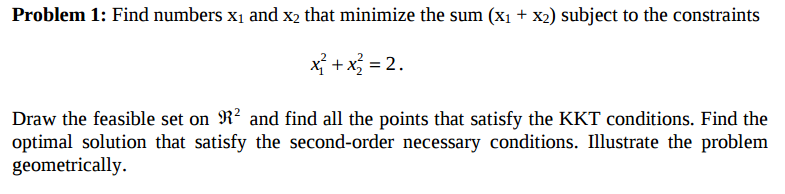
\includegraphics[width=0.7\linewidth]{screenshot001}
\label{fig:screenshot001}
\end{figure}

According to the task description, we will show the formula of the \textit{c(x)}:
\begin{flalign*}
c(x) = x_1^2 + x_2^2 -2 = 0
\end{flalign*}

The lagrangian function is ($\lambda$ is the lagrangian multiplier):
\begin{flalign*}
L(x, \lambda) = f(x) - \lambda c(x) = x_1 + x_2 - \lambda(x_1^2 + x_2^2 - 2)
\end{flalign*}

Now we will formulate the KKT conditions for the given system:
\begin{flalign*}
\frac{\delta L(x,\lambda)}{\delta x_1} = 1-\lambda x_1 \triangleq 0,\ then\  x_1 = \frac{1}{2\lambda}\\
\frac{\delta L(x,\lambda)}{\delta x_2} = 1-\lambda x_1 \triangleq 0,\ then\  x_2 = \frac{1}{2\lambda}
\end{flalign*}
The c(x) function, subject to calculated x, shall be zero:
\begin{flalign*}
x_1^2 +x_2^2 -2 = 0\\
(\frac{1}{2\lambda})^2 + (\frac{1}{2\lambda})^2 -2 = 0\\
\\
\lambda^2 = \frac{1}{4}
\\
\lambda = \frac{1}{2} \lor \lambda = -\frac{1}{2}
\end{flalign*}
Now we are calculating both $x_1\ and\ x_2$ according to lambda:
\begin{flalign*}
x = \begin{bmatrix}
1\\
1
\end{bmatrix}\\
x = \begin{bmatrix}
-1\\
-1
\end{bmatrix}
\end{flalign*}

Now to establish the min condition:
\begin{flalign*}
\min_x \{x_1+x_2\}\\
\\
for x = \begin{bmatrix}
1\\
1
\end{bmatrix}&:x_1+x_2 = 2\\
for x = \begin{bmatrix}
-1\\
-1
\end{bmatrix}&:x_1+x_2 = -2\\
\\
\end{flalign*}
Hence, the solution is:
$x = \begin{bmatrix}
-1\\
-1
\end{bmatrix}$

\begin{figure}[h]
\centering
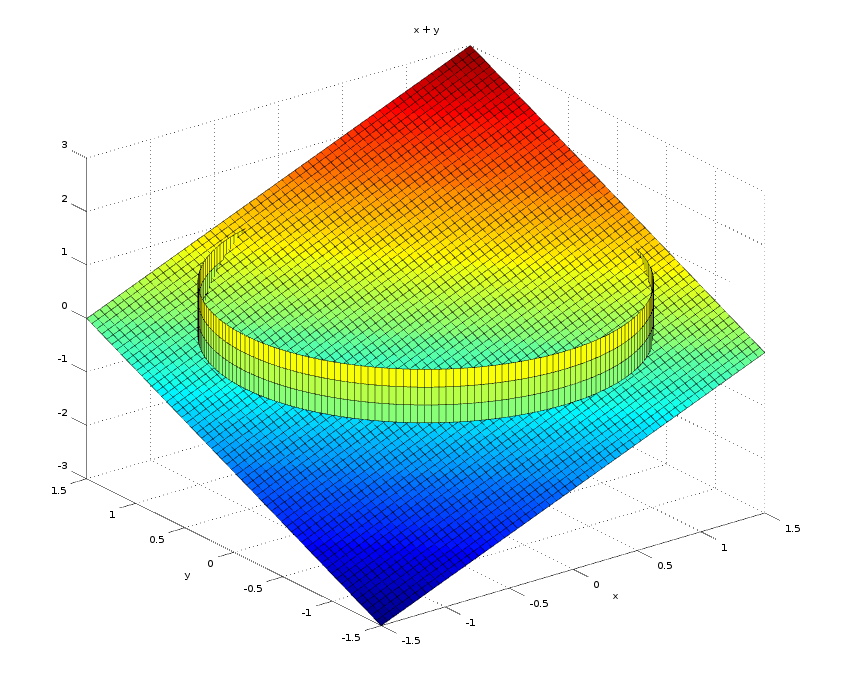
\includegraphics[width=0.7\linewidth]{screenshot002}
\caption{The graphical interpretation of given problem (cylinder of radius $\sqrt2)$ and the plane x+y ($x_1 + x_2$). The solution is in point [-1,-1] - the lowest point in Z-axis that is intersection of the mentioned two surfaces.}
\label{fig:screenshot002}
\end{figure}

The following code was used to illustrate the problem:
\begin{lstlisting}
pkg load symbolic

syms x y;

ezsurf (@(x, y) x + y, [-1.5 1.5 -1.5 1.5])
hold
[X, Y, Z] = cylinder([sqrt(2) sqrt(2) sqrt(2) sqrt(2)],200);
surf(X,Y,Z); 

\end{lstlisting}
\clearpage

%task2
\clearpage

%task3
\clearpage




%task4
\clearpage


%task6
\clearpage



%task7
\clearpage








\clearpage
\chapter{Listings of algorithms}
\section{Coded selected algorithms}
Algorithm 1 - \\ 
\begin{lstlisting}

\end{lstlisting}
\newpage
Algorithm 2 - \\
\begin{lstlisting}
\end{lstlisting}
\begin{thebibliography}{8}
\addcontentsline{toc}{chapter}{Bibliography}
%\addcontentsline{toc}{section}{Literatura}
\bibitem{nocedal}
J. Nocedal, S. J. Wright, Numerical Optimization, Springer, 1999,
\bibitem{zdunek}
Zdunek R., Optimization Methods - lecture slides.
\bibitem{mathworks}
Mathworks webpage, "Unconstrained Optimization Algorithms", https://www.mathworks.com/help/optim/ug/unconstrained-nonlinear-optimization-algorithms.html
\bibitem{uni}
Nonlinear Programming course webpage, North Carolina State University,
http://www4.ncsu.edu/~kksivara/ma706/
\end{thebibliography}

\end{document}

